\section{The WT-MLP-Lag optimizer}
\label{sec:method}

\mname{WT-MLP-Lag} extends input-whitened \mname{MuonT} into a practical two-sided polar optimizer through two co-designed choices: width-thresholded output preconditioning—retaining dense spectral factors on hidden-width outputs while diagonalizing expanded MLP outputs—and a one-update asynchronous lag that moves post-backward output processing off the critical path.

\subsection{Two-sided preconditioned Muon update}
\label{sec:operator}

We consider pre-RMSNorm SwiGLU Transformer blocks with hidden width $\dm$ and MLP expansion width $\dff=4\dm$. Each block contains seven 2D linear projections $y=W_{p,t}x$ with weight matrix $W_{p,t}\in\R^{m_p\times n_p}$: four square attention projections (\texttt{q,k,v,o} of shape $\dm\times\dm$), two tall expansion projections (\texttt{gate,up} of shape $\dff\times\dm$), and one wide contraction projection (\texttt{down} of shape $\dm\times\dff$). Given the globally averaged stochastic gradient $G_{p,t}\in\R^{m_p\times n_p}$, we maintain Nesterov momentum
\begin{equation}
 M_{p,t}=\mu M_{p,t-1}+G_{p,t},\qquad U_{p,t}=G_{p,t}+\mu M_{p,t},\qquad\mu=0.95,
 \label{eq:momentum}
\end{equation}
initialized at $M_{p,-1}=0$, and let $\Nten$ denote the ten-step mixed-precision Newton--Schulz polar map specified in \Cref{app:appendix_math}.

During forward and backward passes over $N_t$ sampled token positions $j$, each projection observes input activations $x_{p,t,j}\in\R^{n_p}$ and backpropagated output cotangents $\delta_{p,t,j}=\partial\ell/\partial y_{p,t,j}\in\R^{m_p}$. We track exponential moving averages of their uncentered second moments:
\begin{align}
 C_{g(p),t}&=\beta C_{g(p),t-1}+(1-\beta)N_t^{-1}\sum_jx_{p,t,j}x_{p,t,j}^{\Tr},\nonumber\\
 B_{p,t}&=\beta B_{p,t-1}+(1-\beta)N_t^{-1}\sum_j\delta_{p,t,j}\delta_{p,t,j}^{\Tr},
 \qquad \beta=0.938,
 \label{eq:moments}
\end{align}
corresponding to an effective horizon of $(1-\beta)^{-1}\approx 16$ updates. Moment sharing is inherently asymmetric between the two sides: because \texttt{q,k,v} share the pre-attention input and \texttt{gate,up} share the pre-MLP input, $g(p)$ collapses forward statistics to four input moments per block (three at width $\dm$ and \texttt{down} at width $\dff$), whereas distinct backward cotangents require seven separate output moments per block (five at width $\dm$ and \texttt{gate,up} at width $\dff$). To remove overall layerwise scale before forming inverse roots, any positive-trace moment $F\in\R^{d\times d}$ is trace-normalized and damped:
\begin{equation}
 \tilde F=\frac{dF}{\tr(F)},\qquad A_d(F)=\tilde F+\epsilon I_d,\qquad\epsilon=10^{-3}.
 \label{eq:trace_norm}
\end{equation}

Using right (input) inner and outer factors $(R_{p,t},\hat R_{p,t})$ built from $C_{g(p),t}$ and left (output) inner and outer factors $(L_{p,t-\tau},\hat L_{p,t-\tau})$ built from $B_{p,t-\tau}$ at staleness lag $\tau\in\{0,1\}$, we update each 2D projection via
\begin{align}
 D_{p,t}&=\hat L_{p,t-\tau}\,\Nten\!\left(L_{p,t-\tau}U_{p,t}R_{p,t}\right)\hat R_{p,t},\nonumber\\
 W_{p,t+1}&=W_{p,t}-\eta_t\left(s_{m_p,n_p}D_{p,t}+\lambda W_{p,t}\hat R_{p,t}^2\right),
 \label{eq:update}
\end{align}
with aspect-ratio scale $s_{m,n}=\sqrt{\max(1,m/n)}$, decoupled weight decay $\lambda=0.1$, and auxiliary AdamW on embeddings, RMSNorm gains, and the untied output head. Setting all four factors to identity recovers \mname{Muon}; setting $L=\hat L=I$ recovers \mname{MuonT}. Here $W_{p,t}\hat R_{p,t}^2$ is \mname{MuonT}'s metric-shaped weight decay from the right reparameterization $W=\widetilde W\hat R$ (\Cref{app:weight_decay}); \Cref{app:left_decay_asymmetry} derives the two-sided counterpart $\hat L^2 W\hat R^2$ and analyzes the structural and experimental-control motivations for retaining one-sided $W\hat R^2$.

\subsection{Width-thresholded factor assignment}
\label{sec:factor_assignment}

Following \mname{MuonT}'s decoupled exponent split, each preconditioned side pairs a $-1/2$ inner whitening factor before $\Nten$ with a unit-RMS $-1/8$ outer scaling factor after $\Nten$, instantiated in either dense spectral ($\mathsf{Dense}$) or coordinate diagonal ($\mathsf{Diag}$) form:
\begin{align}
 R&=A_n(C)^{-1/2},&\hat R&=\unitrms\!\left(A_n(C)^{-1/8}\right),\nonumber\\
 L^{\mathsf{Dense}}&=A_m(B)^{-1/2},&\hat L^{\mathsf{Dense}}&=\unitrms\!\left(A_m(B)^{-1/8}\right),
 \label{eq:dense_roots}\\
 L^{\mathsf{Diag}}&=\Diag(a^{-1/2}),&\hat L^{\mathsf{Diag}}&=\unitrms\!\left(\Diag(a^{-1/8})\right),
 \label{eq:diag_roots}
\end{align}
where $a=m\diag(B)/\tr(B)+\epsilon\mathbf1$ and $\unitrms(X)=\sqrt d\,X/\|X\|_F$ for a $d\times d$ matrix. Scaling outer factors to unit RMS prevents trivial step-size inflation from matrix trace changes; we verify empirical update norms directly on saved checkpoints in \Cref{sec:mechanism}.

\begin{table}[!htb]\centering\small
\setlength{\tabcolsep}{4.0pt}
\caption{\textbf{Factor assignment and nominal output $O(d^3)$ share across core methods.} Dense and Diag denote the $(-1/2,-1/8)$ factor pairs in \Cref{eq:dense_roots,eq:diag_roots}. Splitting both sides by projection role and width ($\dm$ versus $\dff=4\dm$) highlights the structural asymmetry: Muon2-ExpDiag retains dense factors on the $\dff$-wide \texttt{down} input while diagonalizing the two $\dff$-wide gated MLP expansion outputs (\texttt{gate,up}). Fine-grained placement ablations appear in \Cref{tab:ablations}.}\label{tab:taxonomy}
\begin{tabularx}{\textwidth}{@{}>{\raggedright\arraybackslash}Xcccccr@{}}
\toprule
& \multicolumn{2}{c}{Input factors ($R,\hat R$)} & \multicolumn{2}{c}{Output factors ($L,\hat L$)} & & \\
\cmidrule(lr){2-3}\cmidrule(lr){4-5}
Method & $\dm$ (\texttt{attn,o,mlp}) & $\dff$ (\texttt{down}) & $\dm$ (\texttt{q,k,v,o,down}) & $\dff$ (\texttt{gate,up}) & Lag $\tau$ & Out $O(d^3)$ \\
\midrule
Muon & $I$ & $I$ & $I$ & $I$ & --- & 0\% \\
MuonT & Dense & Dense & $I$ & $I$ & --- & 0\% \\
Muon2-Diag & Dense & Dense & Diag & Diag & 0 & 0\% \\
Abl-SymDiag & Dense & Diag & Dense & Diag & 1 & 3.8\% \\
Muon2-ExpDiag (sync) & Dense & Dense & Dense & Diag & 0 & 3.8\% \\
\rowcolor{rowtint}[0pt][0pt]\textbf{Muon2-ExpDiag} & \textbf{Dense} & \textbf{Dense} & \textbf{Dense} & \textbf{Diag} & \textbf{1} & \textbf{3.8\%} \\
Muon2-Dense & Dense & Dense & Dense & Dense & 0 & 100\% \\
Null-Ctrl & Dense & Dense & $I$ (after solve) & $I$ (after solve) & 0 & 3.8\% \\
\bottomrule\end{tabularx}
\end{table}


\mname{WT-MLP-Lag} assigns these operators asymmetrically by side and projection width (\Cref{tab:taxonomy}, \Cref{fig:method_pipeline}(a)):
\begin{itemize}
 \item \textbf{All inputs ($\dm$ and $\dff$):} Dense spectral factors $(R,\hat R)$ on all four input moments, including the $\dff$-wide \texttt{down} input, exactly as in \mname{MuonT}.
 \item \textbf{Hidden-width outputs ($\dm$: \texttt{q,k,v,o,down}):} Dense spectral factors $(L^{\mathsf{Dense}},\hat L^{\mathsf{Dense}})$ to capture cross-channel cotangent correlations, held for one update ($\tau=1$).
 \item \textbf{Expansion-width outputs ($\dff$: \texttt{gate,up}):} Exact per-step diagonal factors $(L^{\mathsf{Diag}},\hat L^{\mathsf{Diag}})$ computed inline without forming $\dff\times\dff$ Gram matrices or eigendecompositions.
\end{itemize}
With five $\dm$-wide and two $\dff$-wide output moments per block, the two expansion outputs account for
\begin{equation}
 \frac{2(4\dm)^3}{5\dm^3+2(4\dm)^3}=96.2\%
 \label{eq:cubic_share}
\end{equation}
of nominal dense output $O(d^3)$ eigendecomposition work and 86.5\% of output Gram storage. Width thresholding therefore eliminates nearly all cubic output-side work while retaining dense spectral conditioning on every hidden-width projection.

\begin{figure}[t]
 \centering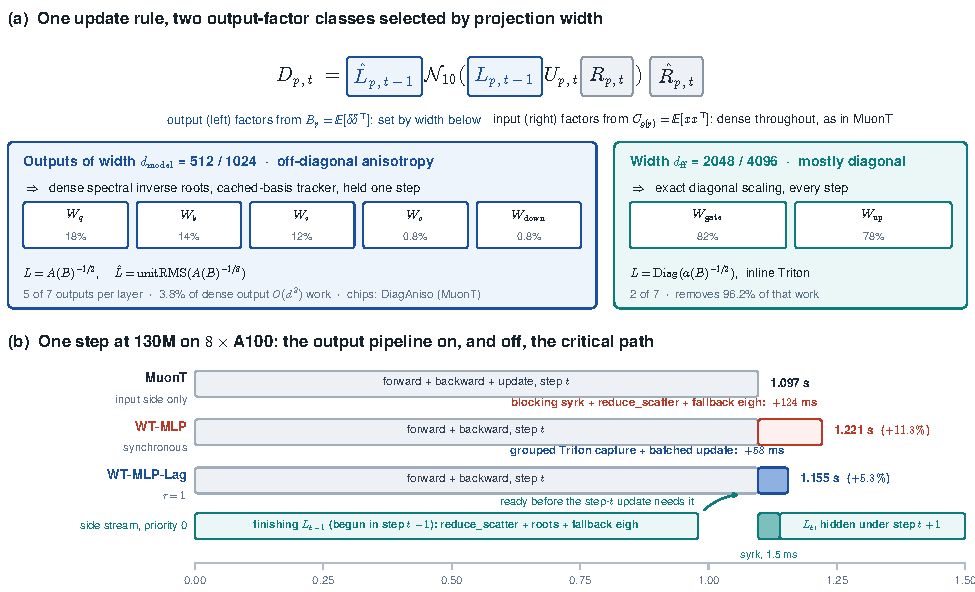
\includegraphics[width=\textwidth]{fig3_method_pipeline.pdf}
 \caption{\textbf{Factor assignment and asynchronous execution pipeline of \mname{WT-MLP-Lag}.}
 \textbf{(a)} Update rule and width-thresholded output classes: dense spectral factors on the five $\dm$-wide outputs (\texttt{q,k,v,o,down}), inline exact diagonal scaling on the two $\dff$-wide expansion outputs (\texttt{gate,up}), and dense input factors throughout. Chip percentages preview each output moment's diagonal share of anisotropy along \mname{MuonT} (\Cref{sec:diagnosis}).
 \textbf{(b)} Single-step execution timeline at 130M scaled to measured eight-A100 medians (\Cref{tab:bench19}). Synchronous \mname{WT-MLP} stalls at the step boundary waiting for output reductions and fallback eigensolves; with a one-update lag ($\tau=1$), \mname{WT-MLP-Lag} applies ready factors immediately while computing new output roots alongside step $t+1$.}
 \label{fig:method_pipeline}
\end{figure}

The inner and outer output factors play distinct geometric roles around $\Nten$. Inner whitening ($L$) changes which output directions dominate the pre-polar singular frame; even when polar orthogonalization normalizes singular values, non-commuting left whitening rotates the resulting orthogonal row frame (\Cref{sec:mechanism}). Post-polar scaling ($\hat L$) subsequently adjusts how much update magnitude is allocated along each output eigendirection. Inherited from \mname{MuonT}, the gentler $-1/8$ outer exponent avoids over-amplifying low-variance cotangent modes and is tested against outer-only and steeper-exponent alternatives in \Cref{sec:controls_ablations}.

\subsection{Asynchronous one-step-lagged execution}
\label{sec:systems}

Forward activations materialize during the forward pass, allowing \mname{MuonT} to overlap input-factor updates with backpropagation. Output cotangents, by contrast, finish arriving only at the end of backward right before the parameter update. To remove output moment reduction and root solving from this critical boundary, \mname{WT-MLP-Lag} sets $\tau=1$ (\Cref{fig:method_pipeline}(b)): step $t$'s parameter update immediately consumes $(L_{t-1},\hat L_{t-1})$ (initialized to identity at $t=0$) together with current input factors, while a priority-0 CUDA side stream contracts, reduce-scatters, and roots step $t$'s captured output statistics underneath step $t+1$'s forward and backward passes. The next update waits only if those background kernels have not yet finished. Although a one-step lag is small relative to the 16-update EMA horizon, we verify directly in \Cref{sec:ablations} that $\tau=1$ preserves nearly all of synchronous \mname{WT-MLP}'s loss improvement.

Three kernel-level optimizations keep statistics capture and dense products lightweight. First, grouped Triton backward hooks capture cotangents at shared autograd nodes; for diagonal \texttt{gate,up} outputs, an inline reduction accumulates squared cotangents directly into FP32 vectors, while dense $\dm$-wide outputs use chunked row buffers that flush partial Grams during gradient accumulation so memory does not grow with microbatch count (permitting larger per-GPU microbatches at 520M). Second, because cotangent eigenspaces rotate rapidly (\Cref{sec:drift_cost}), the cached-eigenbasis root tracker uses GPU-resident residual checks and batched exact fallback eigendecompositions to avoid host synchronization. Third, matching-shape projections share batched update kernels, grouped projections reuse input-factor products, and dense pre- and post-polar matrix multiplications use the FP16-split Tensor-Core arithmetic detailed in \Cref{app:appendix_math}.
